\subsection{Descripción del problema.}

\vspace*{0.3cm}

Dado un tablero de ajedrez de tamaño $n \times n$ y $k$ caballos ocupando
inicialmente ciertos casilleros del mismo, el objetivo del problema consiste
en reunir a todos los caballos en un mismo casillero, minimizando la
cantidad total de movimientos realizados. Esta cantidad equivale a la suma
de los movimientos de todos los caballos en el tablero para llegar a dicho
casillero.

Un caballo puede moverse únicamente respetando los movimientos válidos según
las reglas del ajedrez, pero un casillero puede estar ocupado por más de un
caballo simultáneamente.

\vspace*{0.5cm}

\textbf{Ejemplo:}

En un tablero de 8x8, con 3 caballos en las posiciones [2,2], [5,5] y [2,8],
la menor cantidad de saltos posibles es 4, haciendo que los caballos de los
extremos cayan hacia la posición del caballo del medio[5,5], como se puede ver
en la siguiente imagen:

\begin{figure}[htb]
  \begin{center}
      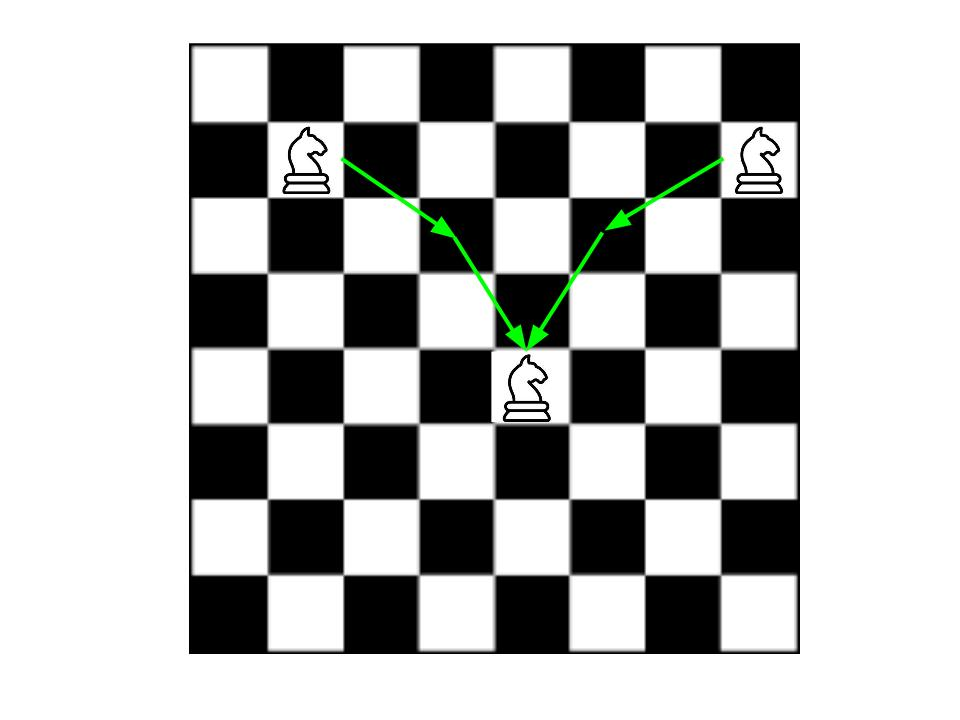
\includegraphics[scale=0.25]{imagenes/caballos.jpg}
  \end{center}
  \caption{ejemplo de tablero.}
\end{figure}


\newpage
\subsection{Desarrollo de la idea y pseudocódigo.}

\vspace*{0.3cm}

Para resolver este problema, utilizaremos $k$ tableros de $n \times n$
casilleros, uno por cada caballo. En cada tablero se calculará el costo para
dicho caballo de llegar a cada casillero, aplicando \textit{BFS} desde el
casillero inicial, quedando inválidos los casilleros que no pueden
alcanzarse.

Luego se recorren todos los casilleros, sumando el valor de estos en todos
los tableros (si son alcanzables), obteniendo así el costo de cada casillero
para cada caballo. De existir, el mínimo de estos valores será el casillero
que pueden alcanzar todos los caballos en la menor cantidad de saltos.

\begin{codebox}
\Procname{$\proc{puntoDeEncuentro}(caballos, n)$}
\li $\id{tableros} \gets \emptyset$
\li \For $caballo \in caballos$ \Do
\li   $\proc{agregar}(tableros,
                      \proc{llenarTablero}(\proc{crearTablero}(n),
                                           caballo))$
    \End
\li $\id{i} \gets 0$
\li $\id{j} \gets 0$
\li $\id{min_i} \gets \infty$
\li $\id{min_j} \gets \infty$
\li $\id{min} \gets \infty$
\li \While $\id{i} < \id{n}$ \Do
\li   \While $\id{j} < \id{n}$ \Do
\li     $\id{sum} \gets 0$
\li     $\id{caballo} \gets 0$
\li     \For $tablero \in tableros$ \Do
% \li       \If $tablero_{ij} \isequal \infty$ \Then
% \li         $\id{sum} \gets \infty$
% \li       \ElseIf $sum \neq \infty$ \Then
\li         $\id{sum} \gets \id{sum} + tablero_{ij}$
%           \End
        \End
\li     \If $sum < min$ \Then
\li       $\id{min} \gets \id{sum}$
\li       $\id{min_i} \gets i$
\li       $\id{min_j} \gets j$
        \End
\li   $\id{j} \gets \id{j} + 1$
      \End
\li $\id{i} \gets \id{i} + 1$
    \End
\li \Return $(\id{min}, \id{min_i}, \id{min_j})$
\end{codebox}


\begin{codebox}
\Procname{$\proc{crearTablero}(n)$}
\li \Return matriz de $n \times n$ inicializada en $\infty$
\end{codebox}


\begin{codebox}
\Procname{$\proc{llenarTablero}(tablero, inicio)$}
\li $\id{posiciones} \gets \emptyset$
\li $\proc{encolar}(posiciones, (inicio, 0))$
\li \While $\lnot \proc{vacio?}(posiciones)$ \Do
\li   $\id{pos} \gets \proc{primero}(\proc{frente}(posiciones))$
\li   $\id{nivel} \gets \proc{segundo}(\proc{frente}(posiciones))$
\li   $\proc{desencolar}(posiciones)$
\li   $\id{i} \gets inicio_i$
\li   $\id{j} \gets inicio_j$
\li   \If $tablero_{ij} \isequal \infty$ \Then
\li     $\id{tablero_{ij}} = nivel$
\li     \For $\id{v} \in \proc{vecinos}(tablero, posicion)$ \Do
\li       $\proc{encolar}(posiciones, (v, nivel + 1))$
        \End
      \End
    \End
\end{codebox}

\newpage
\subsection{Justificación de la resolución y demostración de correctitud.}

\vspace*{0.3cm}

La solución es el mínimo número de movimientos entre todos los caballos que
los deja en el mismo casillero, y la posición de ese casillero. Es decir, si
$s \in [1, \dots, n] \times [1, \dots, n]$ es solución, $s$ pertenece a
\begin{align*}
\min_{(i, j) \in [1, \dots, n] \times [1, \dots, n]} \sum_{c \in caballos}
\text{camino\_mínimo}(c, (i, j))
\end{align*}

Primero completamos, en un tablero para cada caballo, los caminos mínimos
desde la posición inicial de este hasta cada casillero que puede alcanzar.
Para esto, usamos el tablero como un grafo, considerando cada casillero como
un nodo y los posibles saltos de caballos como aristas. Empezando desde la
posición del caballo, se recorren todos los nodos alcanzables mediante el
algoritmo BFS, logrando de esta manera poner la cantidad mínima de saltos
para cada casillero alcanzable, pues BFS obtiene los caminos mínimos desde
un nodo inicial a cualquier otro nodo del grafo, siempre y cuando estos se
encuentren en la misma componente conexa.

Luego de obtener este resultado, para obtener el valor mínimo y la
coordenada donde se alcanza, se recorren todos los casilleros y se calcula
la sumatoria de costos de ese casillero en el tablero correspondiente a cada
caballo. En cada caso se compara el valor obtenido con el mínimo actual y se
actualiza este valor y la coordenada, de ser necesario.

El valor obtenido, si existe, es una solución óptima que minimiza el número
de movimientos de todos los caballos para llegar a ese casillero, pues el
algoritmo es exhaustivo: recorre todos los posibles resultados y se queda
con el menor.

\newpage
\subsection{Análisis de complejidad.}

\vspace*{0.3cm}

\textbf{Aclaraciones} : Se considerará $k$ = cantidad de caballos
 y $n$ = cantidad de casilleros de alto o largo (es indiferente ya que los
 tableros serán cuadrados).

\begin{enumerate}

 \item Las operaciones sobre el contenedor \verb|vector| de la STL (push_back, 
 begin y end) y la creación de sus iteradores toman $O(1)$.
 
 \item En la función \verb|main| la estructura \verb|for| es ejecutada
  $k$ veces, donde se realiza un \verb|make_pair| y un \verb|push_back| 
  sobre un \verb|vector| que cuestan $O(1)$, dando una complejidad de $O(k)$.
   
 \item Crear la esctructura \verb|pair| $respuesta$ que contrendrá el 
 resultado del problema, si lo hay, cuesta $O(1)$.
 
 \item En la función \verb|punto_de_encuentro| se crea el \verb|vector| 
 $tableros$ ( $O(1)$ ), y con un iterador se recorre el \verb|vector| $caballos$ en 
 $O(k)$ donde por cada iteración se crea un tablero (ver \textbf{Tablero}) 
 en $O(n^{2})$, se crea un \verb|queue| para los casilleros ( $O(1)$ ), 
 se crea un \verb|make_pair| ( $O(1)$ ) y se los inserta en el \verb|queue| $casilleros$
 mediante \verb|push| ($ O(1)$ ), se llena el tablero creado (ver \textbf{LLenar tablero}) 
 en $O(n^{2})$ y se los agrega a $tableros$ con \verb|push_back| en $O(1)$
  dando una complejidad total de $O(k.(n^{2} + n^{2}))$ = $O(k.n^{2})$.
 
 \item \textbf{Tablero} - Crear un tablero implica crear un \verb|vector| 
 que contendrá otro \verb|vector| dentro ($O(1)$) y se le dará tamaño $n$
 al vector contenedor con \verb|resize| en $O(n)$. Luego se creará un iterador
 ($O(1)$) para recorrer el \verb|vector| contenedor ($O(n)$) y en cada iteración
 al \verb|vector| contenido en dicha posición se le seteará $n$ posiciones
 en $-1$ ($O(n)$), dando una complejidad total de $O(n^{2})$.
 
 \item \textbf{Llenar tablero} - La función posee un \verb|while| donde se ejecutan
 todas las instrucciones, mientras el \verb|queue| $casilleros$ sea diferente de vacío.
 $casilleros$ comienza con 1 elemento y en cada ejecución se le realiza
 \verb|pop| de un elemento y se le agregan todas las posiciones a las cuales se 
 pueden saltar (siguendo el patron del caballo y sin que salga del tablero), la 
 complejidad del \verb|while| sera de $O(n^{2})$ en el peor caso (todos los casilleros), multiplicado 
 por la complejidad de las instrucciones que se ejecuten dentro del mismo.
 
 Crear un \verb|pair| y asignarle el \verb|first| de la tupla del primer elemento 
 de $casilleros$ cuesta $O(1)$, al igual que crear un \verb|int| y asignarle el
 \verb|second| de la tupla del primer elemento de $casilleros$.
 
 Hacer \verb|pop| de $casilleros$ cuesta $O(1)$.
 
 En el primer \verb|if| acceder al elemento $[x][y]$ del \verb|vector[vector]| 
 $t.casilleros$ del tablero y compararlo con -1 cuesta $O(1)$ (notar que $tablero$ 
 posee un $casilleros$ \verb|vector[vector]| y que la función $llenar\_tablero$ recibe otro $casilleros$ 
 \verb|queue|). En caso de ser verdadero se realiza un \verb|continue| en $O(1)$.
 
 Asignarle al \verb|int| $nivel$ un elemento de $t.casilleros$ en $[x][y]$ cuesta $O(1)$.
 
 Para las ocho posiciones posibles a las que puede saltar un caballo desde la posición
 actual, validar que la posición sea válida (que caiga dentro del tablero) cuesta 
 $O(1)$, y de ser válida ver si el valor almacenado en dicho lugar es distinto de -1
 también cuesta $O(1)$. Si se cumplen estas condiciones se ejecuta la instrucción 
 del if donde se agrega el casillero que se acaba de evaluar al \verb|queue| $casilleros$
 ($O(1)$) que se recorre en el \verb|while|, realizando dos \verb|make_pair| ($O(1)$) 
 y asignandole el valor del $nivel$ + 1 ($O(1)$).
 
\end{enumerate}

\newpage
\subsection{Experimentación y gráficos.}

\vspace*{0.3cm}

\subsubsection{Test 1 - benchmark caso aleatorio}

\textcolor{red}{\textbf{completar!}}


\newpage
\subsubsection{Test 2 - benchmark del peor caso}

Este ejercicio no tiene mejor y peor caso, todos tardan lo mismo.
Porque en todos los casos se generan los tableros para todos los caballos
y también se busca el mínimo en todos los casilleros.-
\textcolor{red}{\textbf{completar!}}


\newpage
\subsubsection{Test 3 - benchmark del mejor caso}

\textcolor{red}{\textbf{completar!}}
